\chapter{案例分析}
借助第四章描述的多分辨率词云生成方法,我们收集了几例不同性质的数据并生成相应的双分辨率词云,结合真实案例探讨这一可视化形式的参数调整及其有效性。

\section{文学作品}
《全唐诗》是清康熙四十五年由曹寅、彭定求、沈立曾、杨中讷等人奉敕编纂而成,共收录唐代诗人$2,529$人的诗作$42,863$首。我们选定高频双子词作为父文本,其字号直接对应于词频;而子词云则对应运用了该词的诗句。考虑到由于不同的诗在传诵程度上有所区别,而人们自然地对自己所熟知的诗感到亲近,为了增强该双分辨率词云的趣味性,我们假设诗人所收录作品数与其影响力有一定关联,故将其作为子词云的权重,来反映诗句可能的的流行度。

图~\ref{fig:tang_poet}展示了$28$个高频词所对应的部分上下文。可以观察到,《全唐诗》中带有负面情绪的词语偏多,如``不得''、``寂寞''、``惆怅''等,正应了``悲愤出诗人''的古话。而气象相关的词语为最常见的意向,如``明月''、``春风''、``秋风''、``白日''、``白云'',所谓寓情于景,大部分相关诗句虽关乎景,但其怅惘与忧思跃然纸上。

这一数据是\textbf{子文本基数大}的典型案例。由于在词云中,字号已预先指定,而布局中常用的贪心算法会因为布局区域的限制忽略掉重权重较小的词。案例图片展示的是对纸面规格设定较为适宜的词云,在$30cm\sim40cm$的普通阅读距离下即可同时观察双层词云,父词云远至$2m$外依然可辨,文本较为丰富,颇具代表性。但是,这也造成每个子文本区域的平均空间较少,能够放置的词云有限。此外,由于父词云笔触较细,有相当一部分父词云的内部区域未能被子词云填充。一个更好的选择是利用上大型显示设备的高分辨率特性来展示更多的数据,为数据提供全貌。


\section{社交媒体}
我们收集了美国总统唐纳德·约翰·特朗普(Donald J. Trump)自2020年一月一日至2020年五月十五日在社交平台Twitter上的原创发言记录\footnote{\url{https://twitter.com/realDonaldTrump}},共计$1852$条,平均每日约$13$条。我们以高频词语作为父文本,使用点赞数与转发数之和作为父文本的权重,以此反映该词的常用程度以及相关推文受到的关注。

在一般的词云中,关键词往往都非常精炼,从不会超过一行。但是,在双分辨率词云中,有可能存在父文本所对应的上下文或其他类型的子文本文字内容过长的情况,此时若依然维持一字排开会极大降低文本的易读性,距离较近时甚至需要观众移动以完整阅读。因此,在\textbf{子文本内容较长}的情况下,应对文本适当分行,控制近处视图内的文字。我们设置一行的宽度为最大$50$字符,使长句变为文本块。为避免出现两个文段交错布局的现象(参考图~\ref{fig:trump}),我们对算法1进行了适当的调整,将整个文本块视为一个整体,在更新二值矩阵时填充其最小外接矩形而非逐字渲染。

我们分别在普通桌面显示屏规格(图~\ref{fig:trump})和墙面规格(图~\ref{fig:wall})的设定下生成了特朗普推特的双分辨率词云。我们大致可从父文本内容中的名词了解到近半年以来,特朗普的推文多有关总统事务、民主党派、美国、伊朗、就业、新闻等等。而作为形容词的``Fake''使我们不明所以。进一步查看相关推文,我们发现它几乎完全以``FAKE NEWS''的形式出现,指责新闻报道失实,言辞间情绪激动,但并未给出明证与理由,正文末尾多附以超链接。从语言风格来看,特朗普似乎倾向于使用通俗易懂的词汇,且大量使用字母大写和感叹号,特别是对短短几字的推文。``Great''是词频最高的,推文中多次提到``Make America great again''的宣言,其他情况多表示对人事物的赞扬。

尽管《全唐诗》是在小空间下布局,但由于其子文本简短,整体空间利用率较高,疏密得当。但对于具有大块文字的推特数据而言,其在普通桌面显示屏下的效果欠佳。绝大部分父文本及其内部未能为子文本提供布局空间,画面稍显凌乱。这一问题在大屏设定下有所改善。在换用粗笔触字体并提高父子词云字号的差异后,更多空间得到填充,总体布局较为均匀。此外,得益于我们的高频滤波策略,内层子词云与外层子词云之间不存在太强的割裂感,颇为和谐。


\section{双层主题}

2020年5月22日,在第十三届全国人民代表大会第三次会议上,国务院总理李克强发表了《政府工作报告》\footnote{\url{http://www.gov.cn/zhuanti/2020lhzfgzbg}},重点提及了深化改革、扩大内需、脱贫攻坚、对外开放、保障改善民生与政府建设六点。我们以此为线索,人工梳理了发言稿中这六个主题下的子话题,将其可视化。此处相同层次文本的权重具有一定随机性,大致上相同,字号没有特定的指向性。

这一数据属于\textbf{子文本数据有限}的情况。因为父词云字号需要足够大,这会造成子词云可布局空间过大,从而使子词云过于稀疏,不利于集中地观察。此时,我们允许子文本重复出现,得到图~\ref{fig:gov}。这种方式尽最大可能地填满了所有空隙,保证了远处视图的美观。同时,我们设置画布为较小的规格,以避免词语重复过多。

\bigbreak

%\section{小结}
%在对以上数据的分析中,我们对不同规格的画布以及不同双层文本性质下的双分辨率词云进行了讨论,进一步明确了不同设定下的
%\begin{itemize}
%	\item \textbf{}
%\end{itemize}


\begin{figure}[htbp]
	\centering
	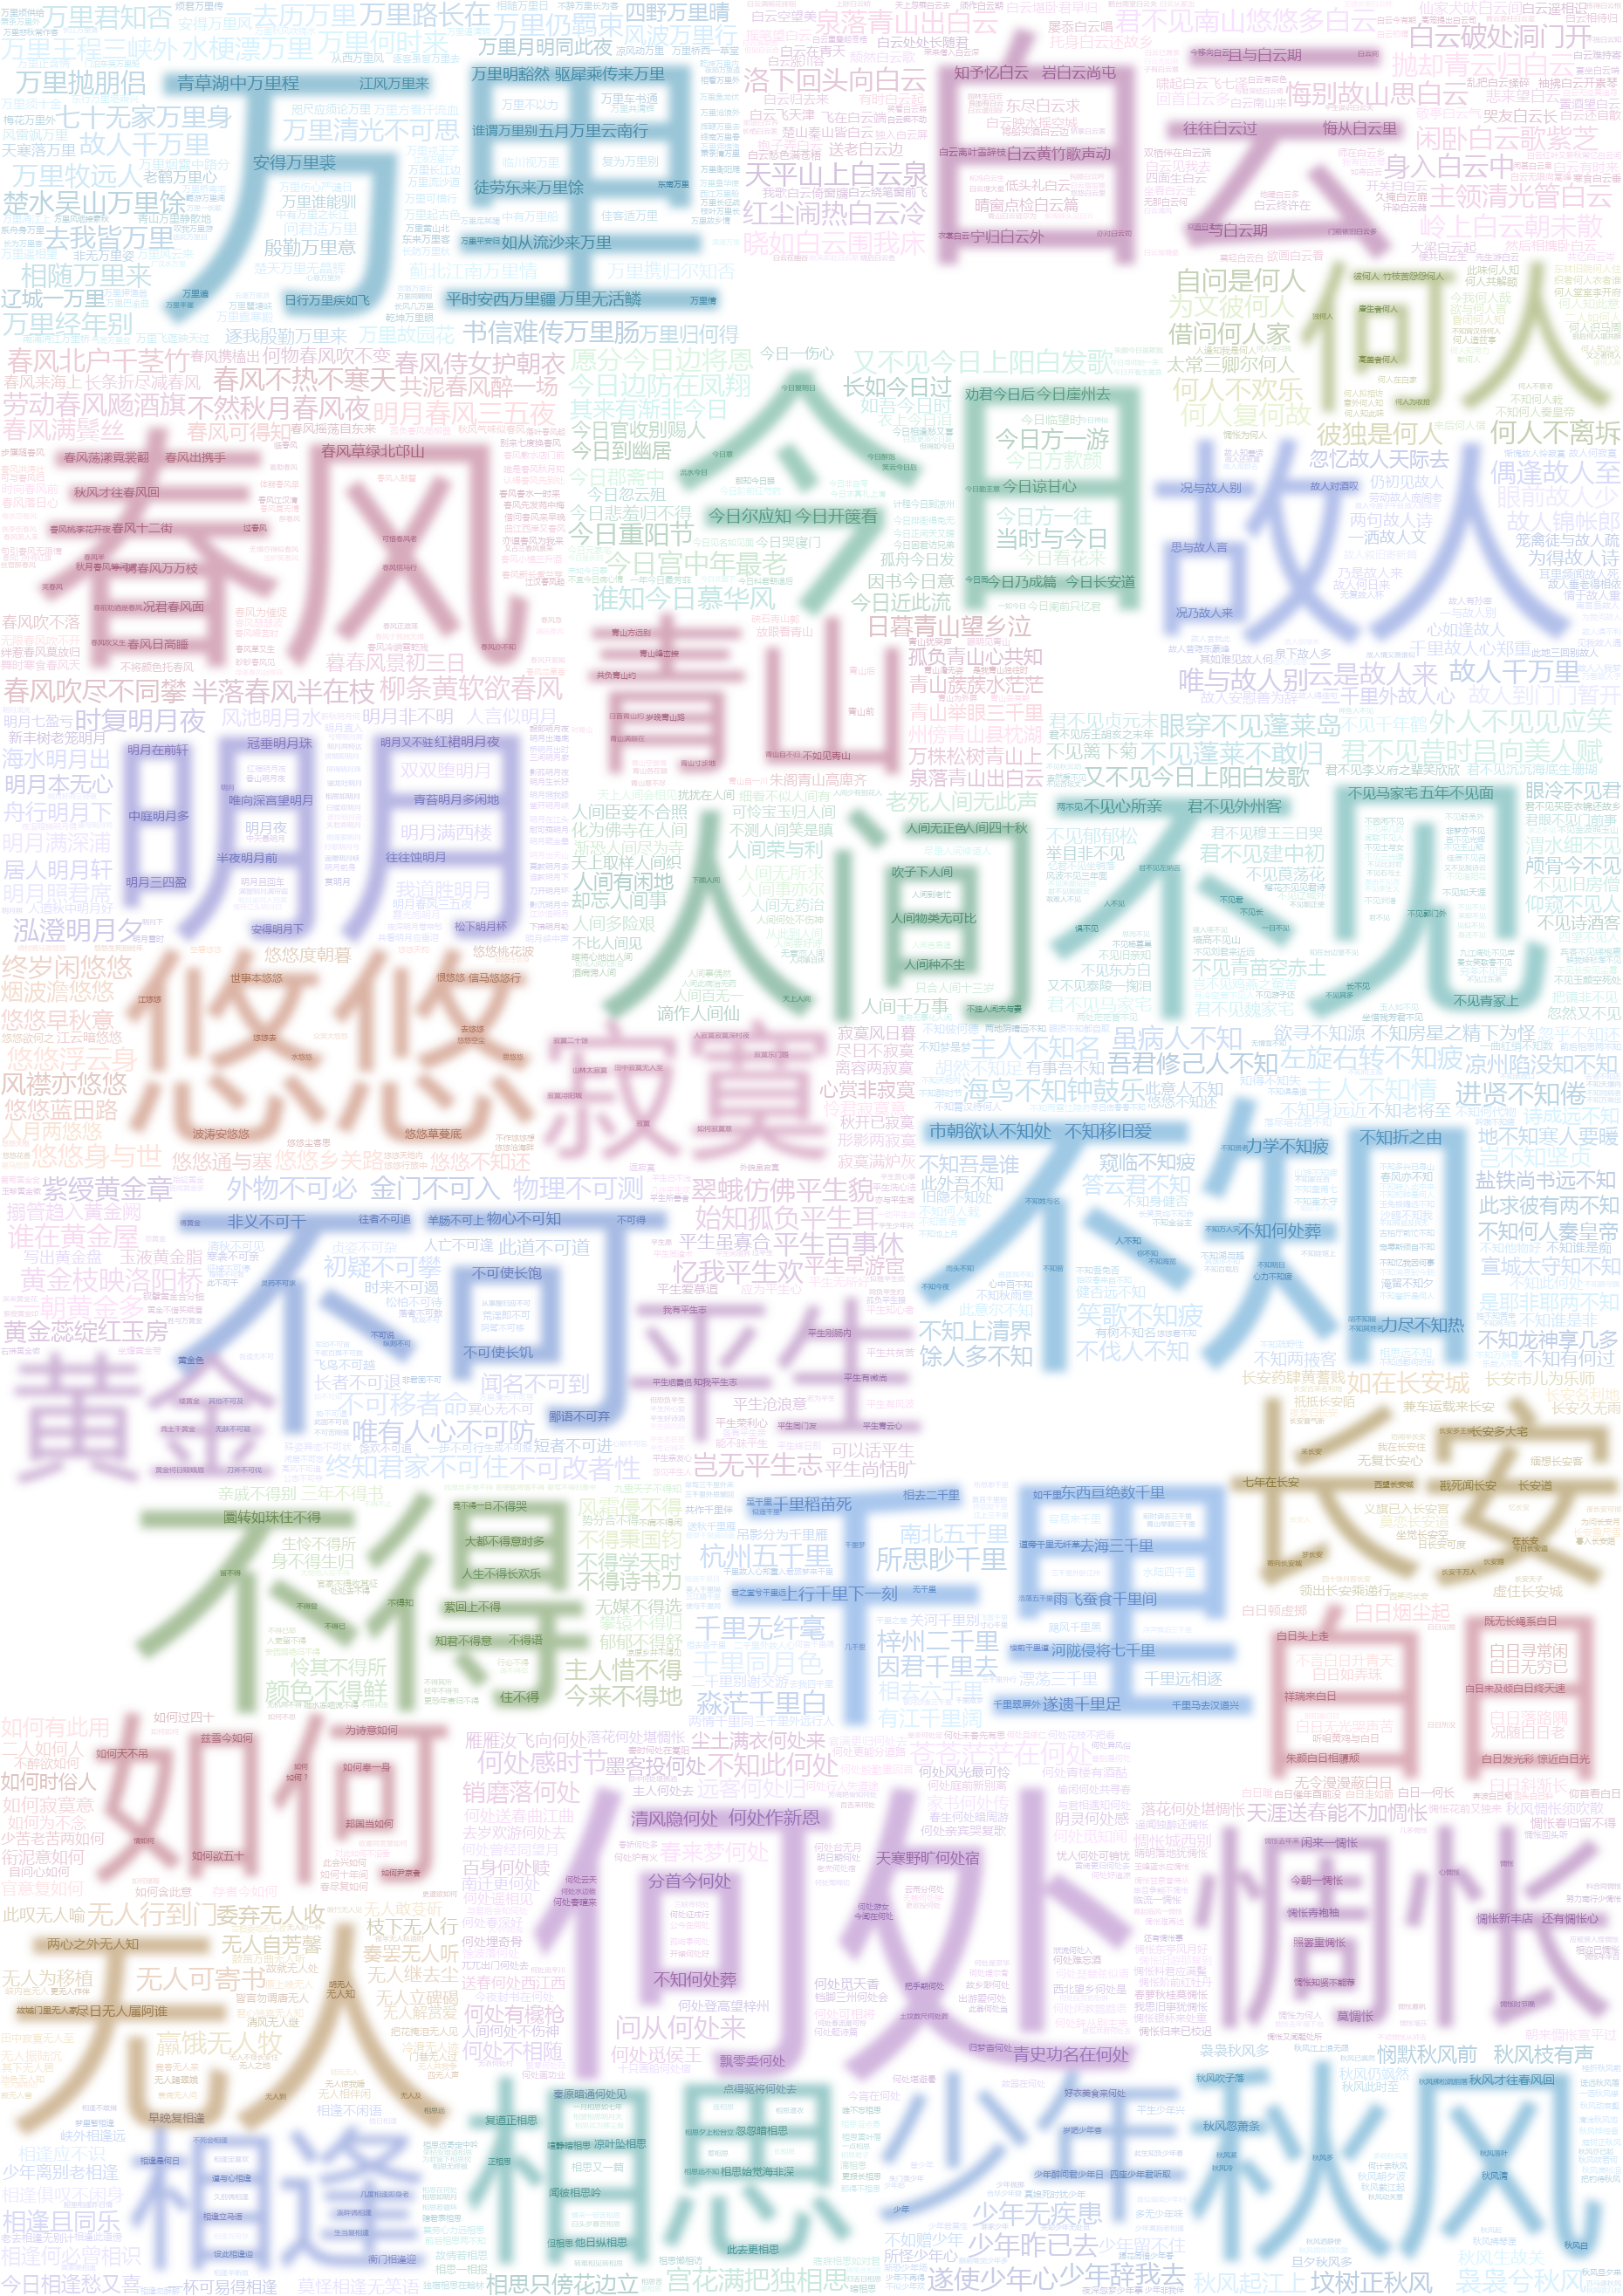
\includegraphics[width=\textwidth]{figures/tang.png}
	\caption{纸面规格:《全唐诗》高频双子词云。}
	\label{fig:tang_poet}
\end{figure}


\begin{figure}[htbp]
	\centering
	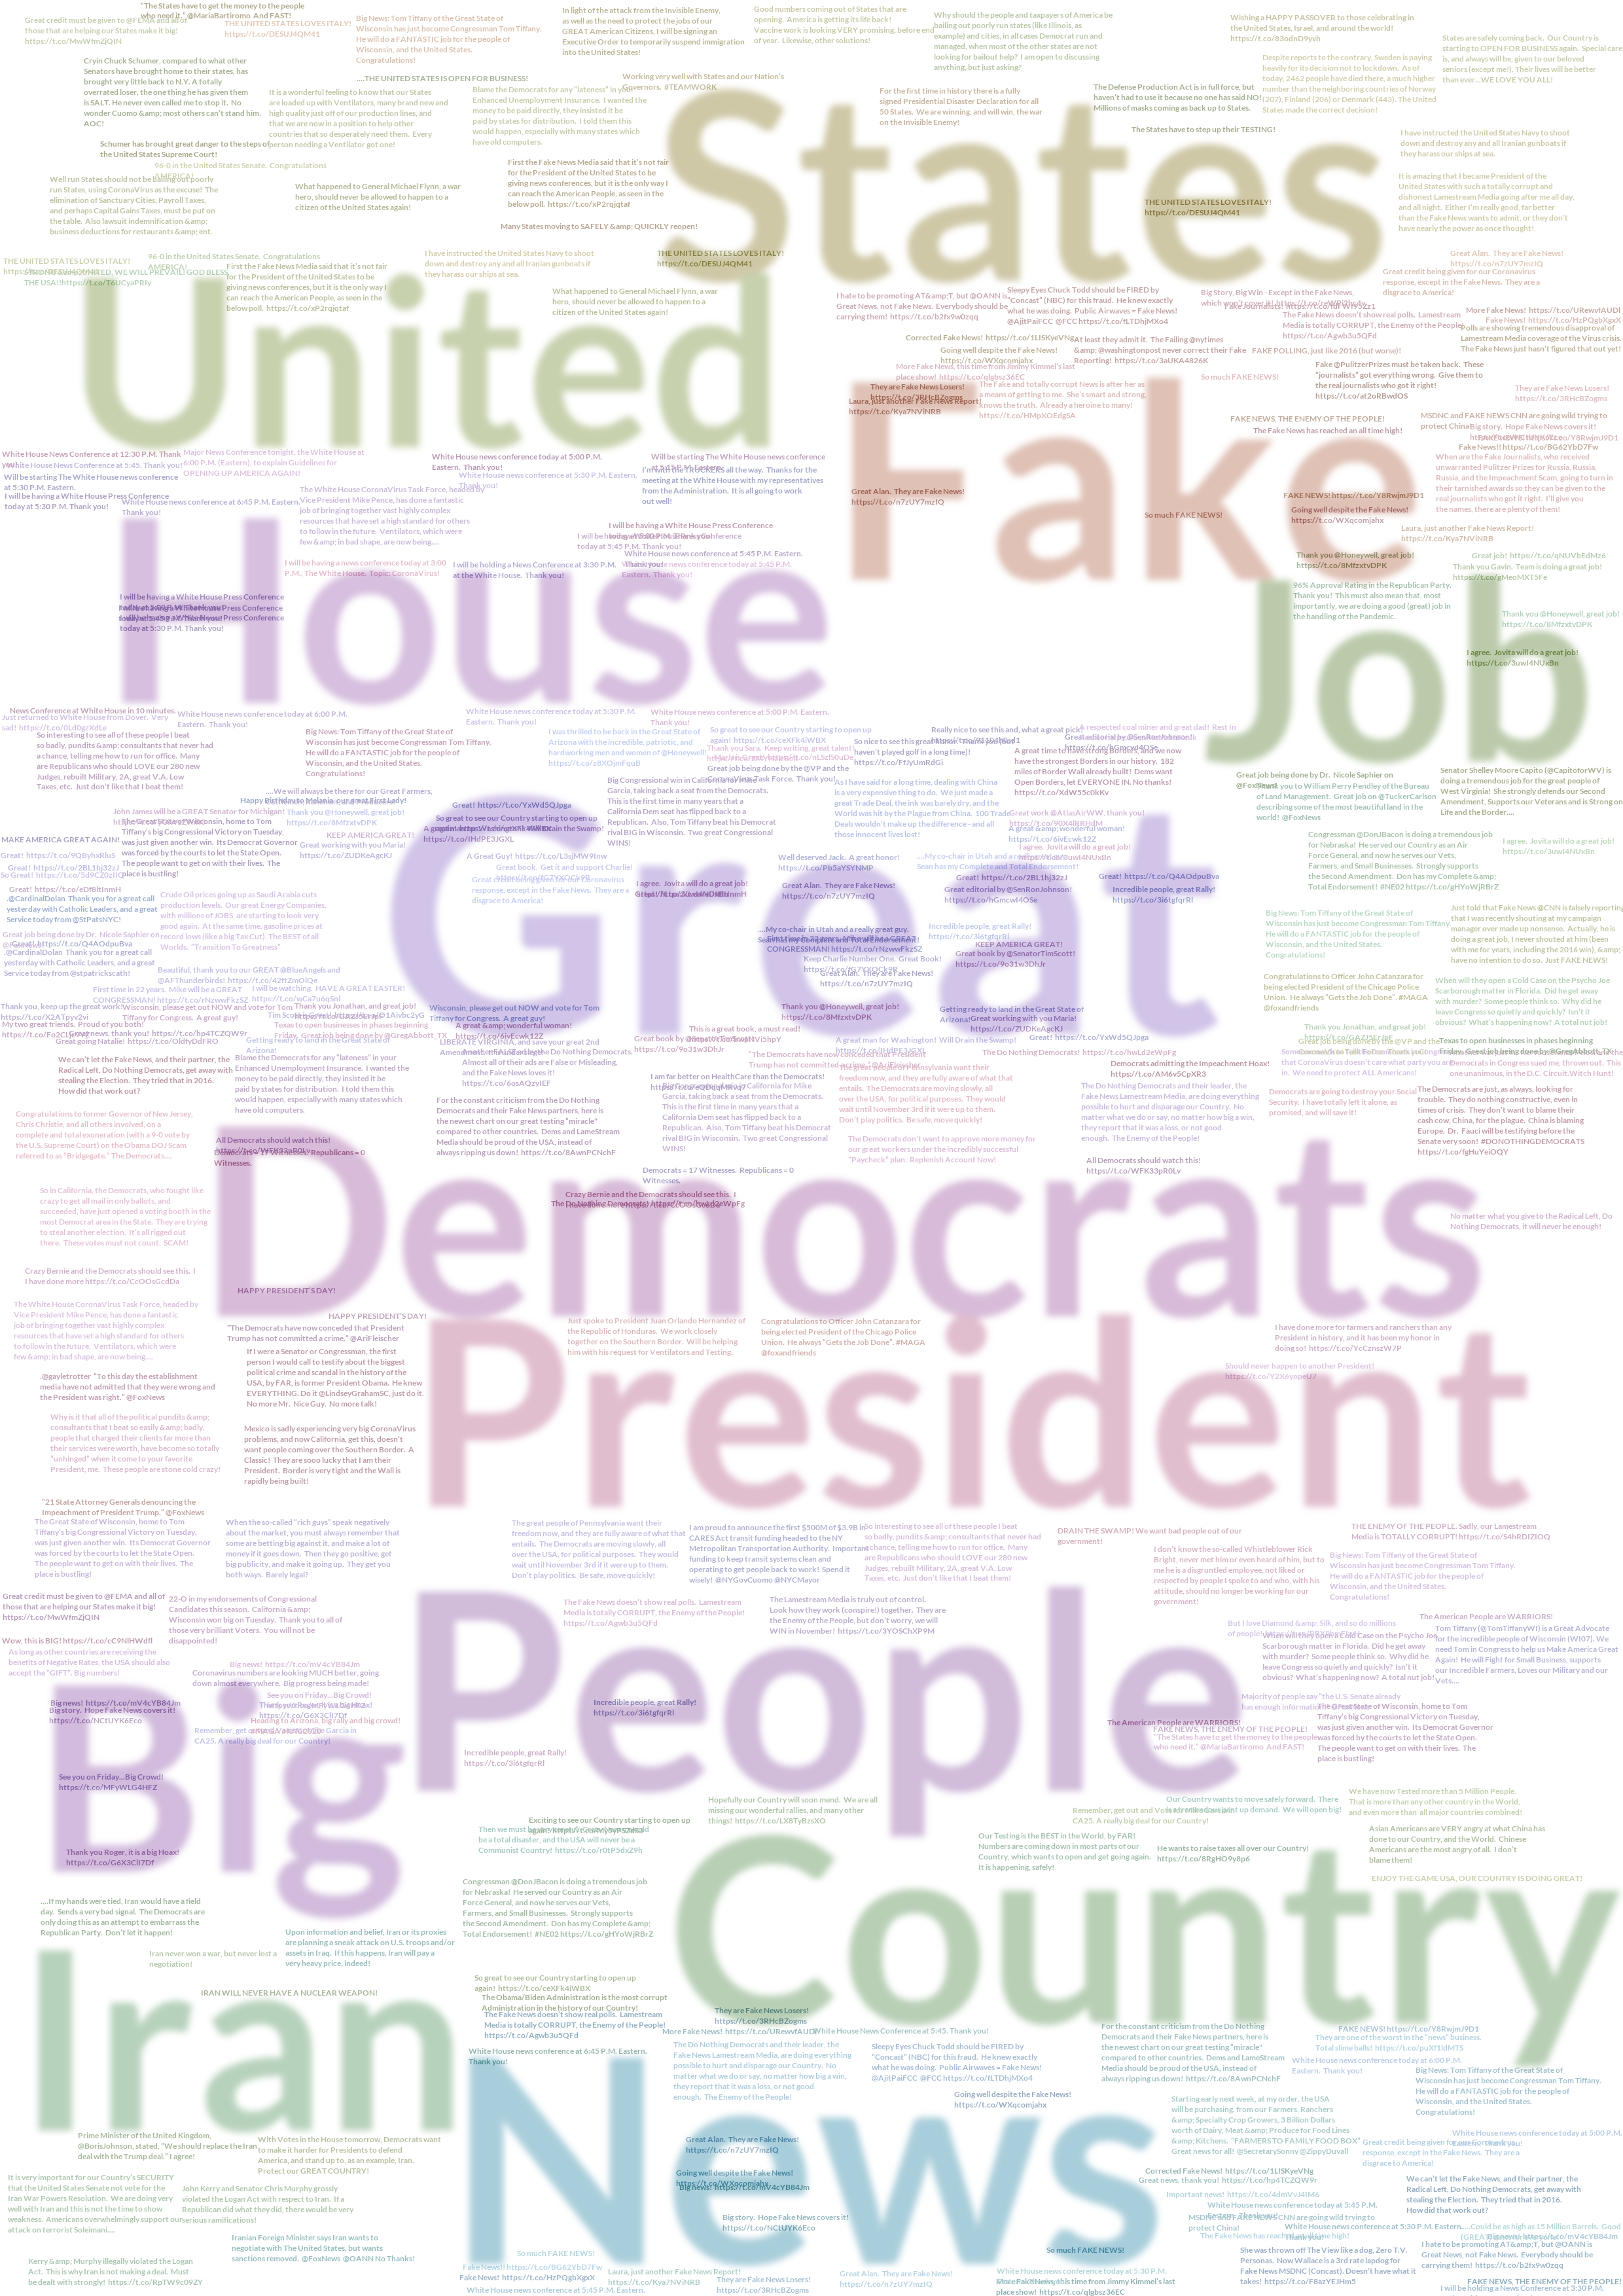
\includegraphics[width=\textwidth]{figures/trump.png}
	\caption{普通显示器规格:特朗普推特发言。}
	\label{fig:trump}
\end{figure}

\begin{figure}[htbp]
	\centering
		
\includegraphics[width=\textwidth]{figures/trump_crop.png}\\
		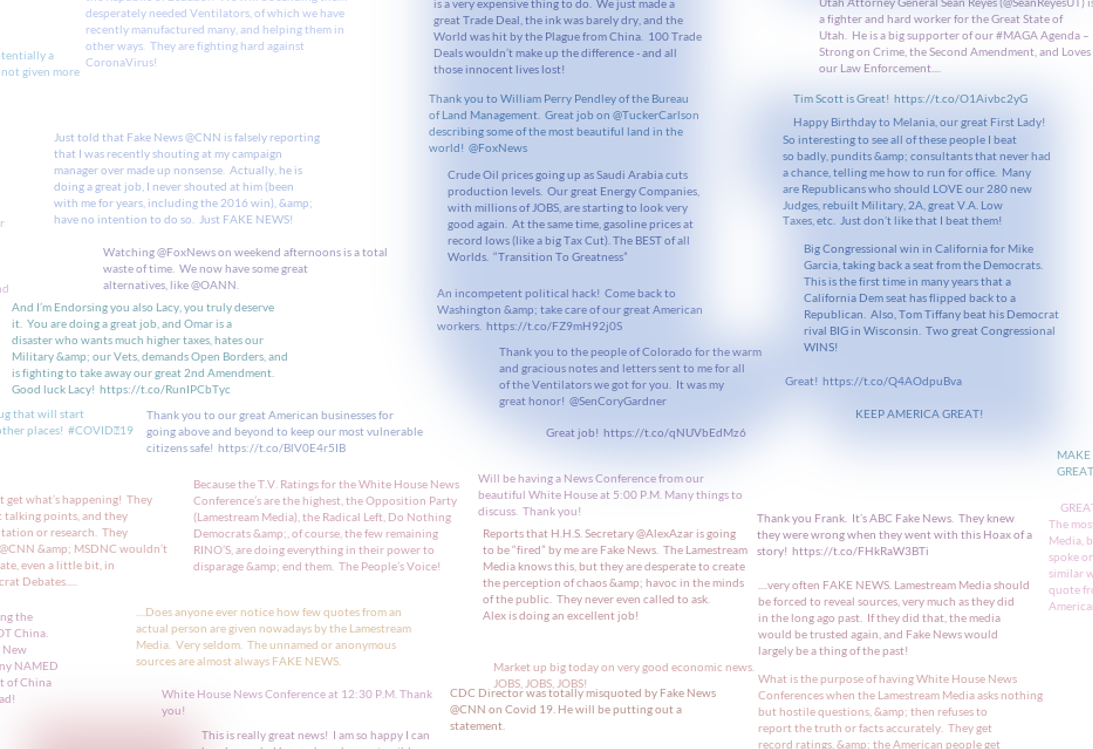
\includegraphics[width=\textwidth]{figures/trump_small.png}

	\caption{墙面规格:特朗普推特发言——概览及细节。}
		\label{fig:wall}

\end{figure}

\begin{figure}[htbp]
	\centering
	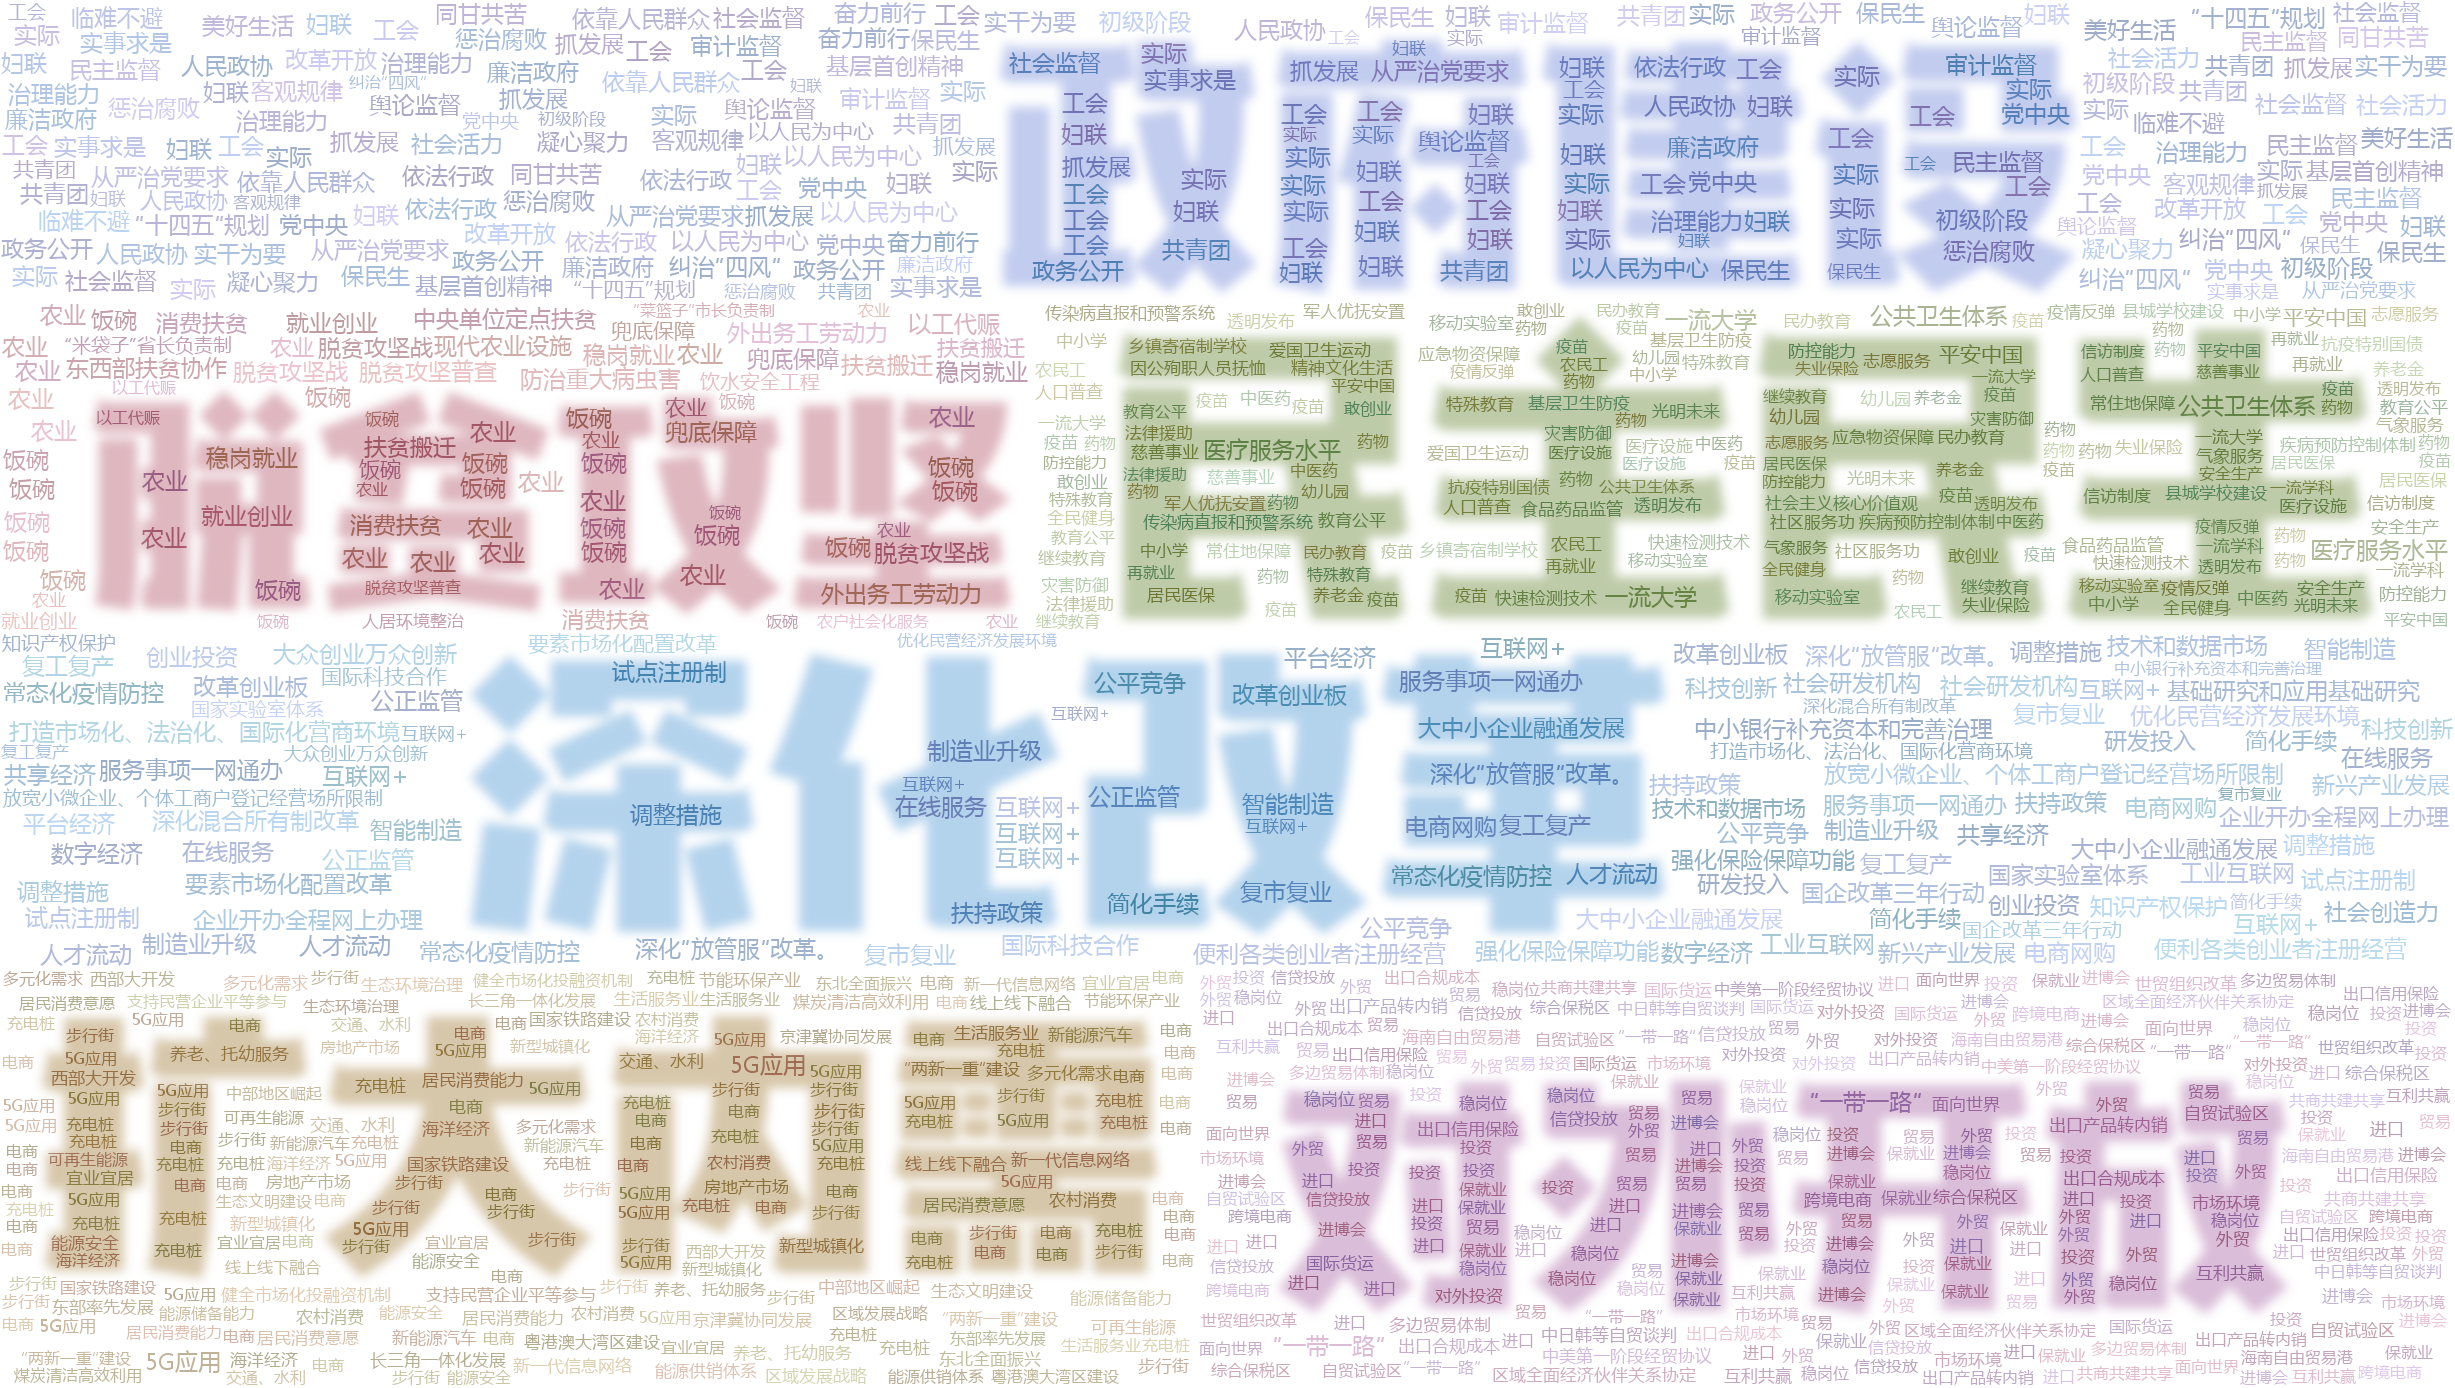
\includegraphics[height=0.95\textheight]{figures/gov_paper.png}
	\caption{纸面规格:2020年政府工作报告。}
	\label{fig:gov}
\end{figure}
